% Online sync refresh: revised workshop report, 2026-08-29. figure-path-fix
The UCB and $\epsilon$-greedy algorithms were compared on the same
10-armed bandit over a horizon of $T=10^4$, with the experiment repeated
over $M=300$ independent reruns. For each run, cumulative pseudo-regret was
computed as
\[
    \sum_{t=1}^{T}
    \left[
        R^\ast-q^\ast(A_t)
    \right],
\]
and then averaged across reruns. The comparison includes UCB with
$c\in\{0,1,2\}$ and the six $\epsilon$-greedy schedules considered
previously.

\begin{figure}[H]
    \centering
    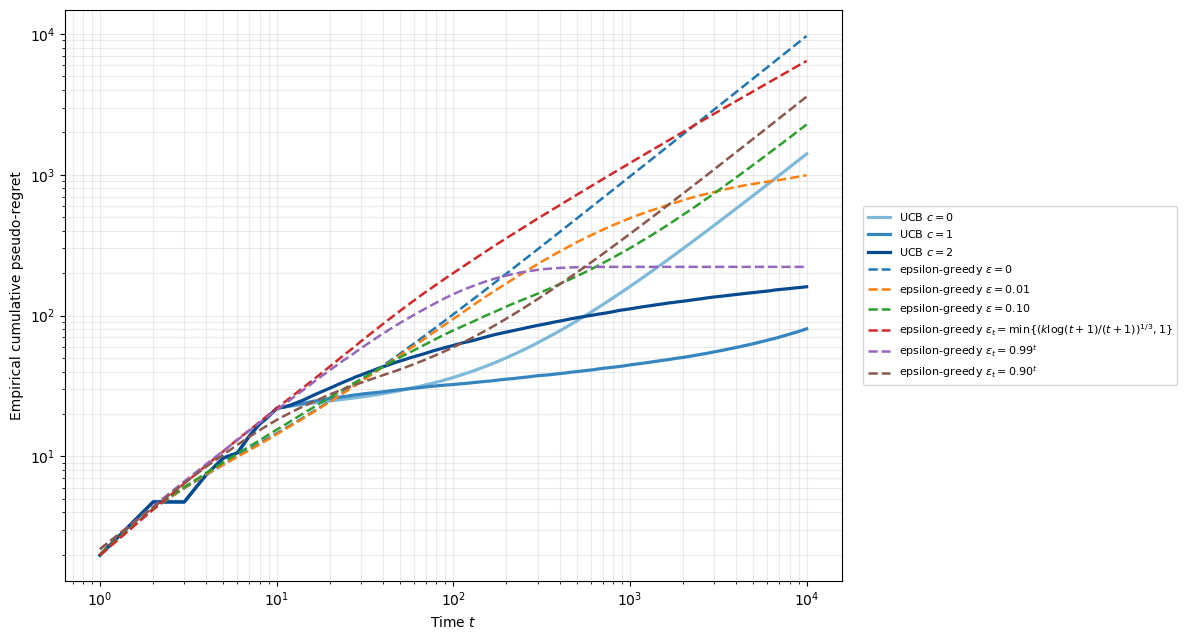
\includegraphics[width=0.82\linewidth]
    {figures/q5_ucb_vs_epsilon_regret.png}
    \caption{Empirical cumulative pseudo-regret of UCB and
    $\epsilon$-greedy algorithms over $T=10^4$ time steps.}
    \label{fig:q5-ucb-epsilon-regret}
\end{figure}

Figure~\ref{fig:q5-ucb-epsilon-regret} shows that the exploratory UCB
algorithms achieve substantially lower finite-horizon regret than the tested
$\epsilon$-greedy policies. At $T=10^4$, the empirical cumulative
pseudo-regret is approximately
\[
    80.6 \quad \text{for UCB } c=1,
    \qquad
    160.3 \quad \text{for UCB } c=2,
\]
whereas the best-performing $\epsilon$-greedy schedule,
$\epsilon_t=0.99^t$, has regret approximately $222.0$.

Among the UCB configurations, $c=1$ gives the lowest regret in this
experiment. Increasing the exploration coefficient to $c=2$ incurs a larger
exploration cost and therefore slightly higher regret, although the results
of Question~4 show that this additional exploration produces more accurate
estimates of the individual arm values. In contrast, $c=0$ does not perform
systematic exploration and incurs substantially larger regret
($\approx 1408$).

The fixed $\epsilon$-greedy policies also accumulate considerably more
regret: at $T=10^4$, the regret is approximately $994$ for
$\epsilon=0.01$ and $2278$ for $\epsilon=0.10$. Persistent random
exploration continues to select suboptimal arms even after the optimal arm
has been identified. The polynomially decaying schedule has even larger
finite-horizon regret ($\approx 6445$), because it continues to explore
aggressively at this horizon. Its longer-run growth is assessed using the
multi-horizon diagnostics interpreted in Question~3.

Therefore, for this bandit instance and finite horizon, UCB provides the
best exploration--exploitation trade-off: its uncertainty-directed
exploration identifies the optimal arm with substantially less unnecessary
exploration than the tested $\epsilon$-greedy policies.
